\subsection{Exemplars} \label{IdeasLabel}
In this section, a current IT-system will be described and what other systems that can be used to plan what food to eat.
Ideas from other existing systems will be found and put into the context of this projects system. \fxnote{CHS: Still don't know how or if, to incorporate metaphors}s

\subsubsection{Food Planner}
One technology that are currently being used to make a food plan is a mobile application called \textit{Food Planner}.
In this application the users can plan meals ahead of time, lookup recipes, look at what groceries that needs to be bought, list what the user have in the fridge and appends bought items to the fridge.
The following section will take a look at the application, in order to find ideas which will be good in the context of this projects system.

\begin{figure}[H]
    \centering
    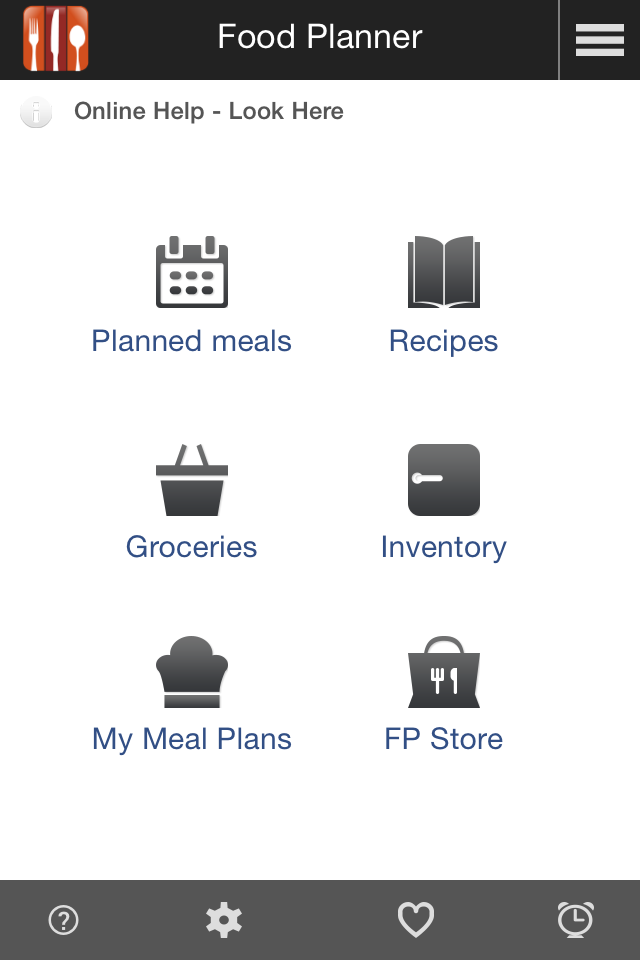
\includegraphics[width=0.5\textwidth]{Grafik/FoodPlanner/index}
    \caption{An image displaying the index of the application Food Planner}
    \label{FoodPlannerIndex}
\end{figure}

\textbf{Useful ideas:}
\begin{itemize}
  \item \textbf{Inventory:} Each product can be added separately, and the application can be used to keep track on the amount
  \item \textbf{Recipes:} Custom recipes can be created through the application, or they can be found/bought in the application store, or the internet, either by a Google search, or following a link directly to known websites, with recipes.
  \item \textbf{My meal plans:} This menu can keep track of meal plans, that has been added to the application.
  \item \textbf{Planned meals:} In this menu the upcoming days can be planed, with multiple recipes each day, either by adding them manually, or by adding a meal plan from \textit{My meal plans}. Missing groceries for a desired number of days ahead, can then automatically be added to a \textit{Grocery menu}.
  \item \textbf{Registering:} By registering with an e-mail and a password, the application allows the user to back up the information, synchronizing with other devises and sharing is also enabled.
  \item \textbf{Grocery menu:} Here, groceries that needs to be bought, can be added either automatically from \textit{My meal plan} or added manually. If an item is not known to the program, it can be added using a bar-code scanner, and naming the item manually.
\end{itemize}
\fxnote{"Should I add more pics of Food Planner app?" Christian asked the group.}

\textbf{Ideas used in the context of a new program}
\begin{itemize}
  \item \textbf{Inventory:} To help avoiding food waste, this idea would be useful. By prioritizing the inventory, the food in the home, has a better chance of being used, before it expires.
  \item \textbf{Recipes:} Using Recipes, people can try new meals, and if the ingredients list, needed for the meal is known, the Inventory can be taken into account, or a list of needed ingredients can be added to the grocery menu.
  \item \textbf{My meal plans:} With this idea, it is easy to save different diets, and lists of favourite meals, etc.
  \item \textbf{Planned meals:} Knowing what food is planned ahead, new recipes can be added to reduce food waste and/or variate the meals.
  \item \textbf{Registering:} This idea enables the use of synchronizing, which could be useful if the program is used in a household of more than one, or if it is to be used on multiple devices.
  \item \textbf{Grocery menu:} This menu is very useful, for the use of a shopping list, where it can be tracked what has been bought and what still needs to be bought.
\end{itemize}


\subsubsection{Website\fxnote{To be rewritten, do not read yet!}}
Another alternative could be a tool found on the website http://realfood.tesco.com/meal-planner.html\cite{tesco_foodplan}. The website has six main menus; About meal planner\footnote{What we call \textit{food plan}, the website calls meal plan. This report will from here on, use food plan where the website uses meal plan.}, Create your own, Leftover inspiration, Featured food plans, Customer food plans and My binder, for now these menus will not be explained, but they have been looked through, to find useful ideas, before its looked upon, how they can be used in the context of a new program.

\textbf{Useful ideas:}
\begin{itemize}
  \item \textbf{Meals:} When creating a food plan, the user can chose to plan breakfast, lunch and/or dinner.
  \item \textbf{Surprise me!:} With this feature, an food plan is automatically created, which is a fast way of planning, if you are not afraid of what you might have to eat.
  \item \textbf{Cooking time:} The user can also define if the cooking time must be 30 minutes or less, 60 minutes or less or if the user does not mind.
  \item \textbf{Dietary preferences:} When creating the plan, the user can also set preferences such as; vegetarian, egg free, gluten free and low fat, furthermore the user can add liked and disliked ingredients, before searching for recipes. Another preference, which can be set here is if the user is on a budget.
  \item \textbf{Leftover inspiration:} The website offers features to lower food waste, by having articles on how to use leftovers and cook meals so they are easy to save for another day. Lastly they have an option to list leftovers and then recommend recipes from this list.
  \item \textbf{Featured plans:} It is possible to browse the websites featured food plans, either for inspiration, or to add the entire food plan, to your own.
  \item \textbf{Customer plans:} In this menu the users, or customers, of the website can add their own food plans or browse other users food plans, when browsing, it is possible to filter by; vegetarian, quick and easy, family, dietary preferences, healthy and budget.
  \item \textbf{My binder:} With this menu it is possible to bind recipes and give them notes. The website then offers a feature to search and filter the saved recipes by ingredient, cuisine, dietary requirements and cooking time, if the meal has been cooked yet, or a simple alphabetic order.
\end{itemize}

\textbf{Ideas used in the context of a new program}
\begin{itemize}
  \item \textbf{Meals:}If a user has a company deal including lunch, it will not be necessary to plan lunch, therefore this idea could be optimal to include.
  \item \textbf{Surprise me!:} Is a good function for the user who wants new inspiration and cannot decide on what to have.
  \item \textbf{Cooking time:} Some days are more busy than others, therefore adding this feature would be ideal.
  \item \textbf{Dietary preferences:} If a user would like to follow a specific diet, it would be ideal to let the program help with finding recipes for the specific diet.
  \item \textbf{Leftover inspiration:} This function is ideal to help avoid food waste.
  \item \textbf{Featured plans:} Not having to create all meals on your own or gives new inspiration.
  \item \textbf{Customer plans:} This feature allows for recipes with personal twists, and allow a user to follow custom plans.
  \item \textbf{My binder:} This is an easy way of organizing interesting recipes and food plans. 
\end{itemize}